\lab{Sparse Grids}{spgrid}
\label{lab:spgrid}

\objective{Introduce Sparse Grids.}

\section*{Discretization}
At first inspection, our world appears to be nice and continuous.  However, this only works on a macroscopic level.  As we zoom in on matter, we find that it is made of discrete atoms with much empty space between.  Computers likewise work in discrete space.  You have already seen many examples of this.  Consider plotting the function $y=x^2$, such as in Figure \ref{fig:x_squared}.  To do this we take an array of discrete points of $x$ and $y$ values, which are then joined linearly.  As you either zoom in on the function or decrease the number of plotting points, you can see the discrete nature of even this simple function.

\begin{center}
\begin{figure}
\begin{subfigure}{.49\textwidth}
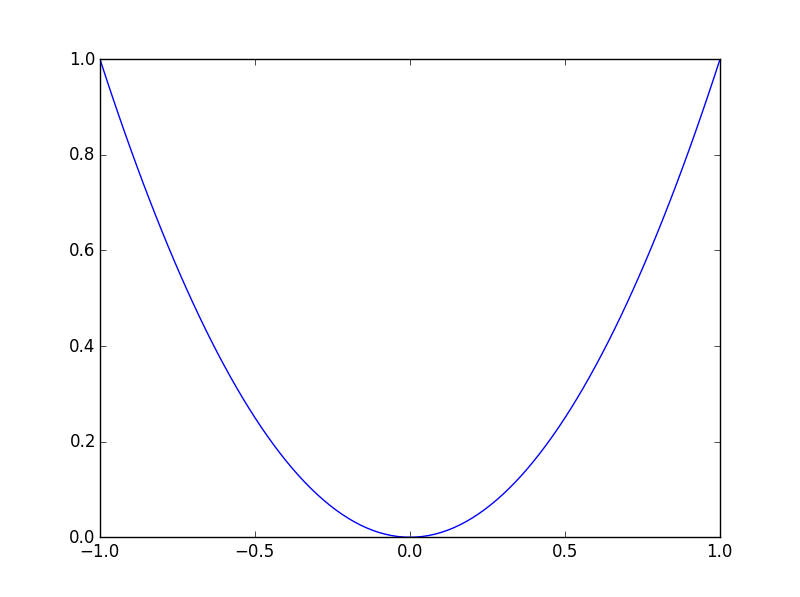
\includegraphics[width=\textwidth]{x2.png}
\end{subfigure}
\begin{subfigure}{.49\textwidth}
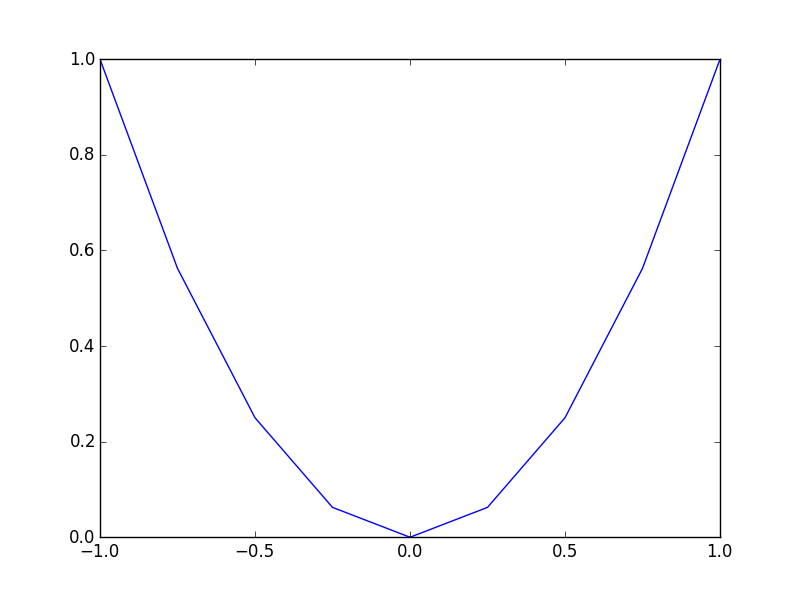
\includegraphics[width=\textwidth]{x2a.png}
\end{subfigure}
\caption{Plots of the function $y=x^2$ using $31$ points and $9$ points, respectively.}
\label{fig:x_squared}
\end{figure}
\end{center}

In order to get better results, we need to use a larger number of points.  This is true not just for graphing purposes, but also for standard computation.  If we double the number of points, we double the computation time necessary.  This effect, while not irrelevant, pales in comparison to the case when working in multiple dimensions.  Imagine a function that we discretize into $20$ points.  A similar function of two variables, where each variable is discretized into $20$ points, would necessitate $400$ unique points.  Expanding to seven variables would necessitate $1,280,000,000$ unique points!

In general, for $n$ discrete points in $d$ dimensions, this gives $n^d$ points.  This can be visualized as a $d$-dimensional grid of size $n \times n \times \cdots \times n$. In practice, we seldom need to know the value for each and every point.  Instead of using the full grid, we can use a sparse grid.  The main idea of a sparse grid is that it can reduce the order of difficulty for a standard $d$-dimensional problem.

\section*{The Hierarchical Basis}
One of the most basic Sparse Grids is based on the use of the \emph{Hierarchical Basis}.  This uses piecewise linear basis functions, the \emph{standard hat function}, to approximate a function.  The standard hat function is defined as:

\begin{equation}
\phi(x) = \left\{
        \begin{array}{ll}
            1-\abs{x} & \quad -1 \leq x \leq 1 \\
            0 & \quad otherwise
        \end{array}
    \right.
\end{equation}

From this equation, we can build a set of basis functions

\begin{equation}
\phi_{j,i}(x) = \phi(2^{j-1}(x+1) - 2i+1))
\end{equation}

\begin{center}
For $j=1$, $i=1/2$.
\end{center}
\begin{center}
For $j>1$, $i=1,2,3,\cdots,2^{j-1}$.  
\end{center}

The first few basis functions are listed in Table \ref{table:functions}, and are plotted in Figure \ref{fig:basis_functions}.

\begin{center}
\begin{table}
\begin{center}
\begin{tabular}{|c|c|c|c|c|}
\hline
$j\backslash i$ & $1$ & $2$ & $3$  & max $i$ \\ \hline
$1$ & $\phi_{1}(x) = \phi(x)$ & & & (1/2) \\ \hline
$2$ & $\phi_{21}(x) = \phi(2x+1)$ & $\phi_{22}(x) = \phi(2x-1)$ & & 2\\ \hline
$3$ & $\phi_{31}(x) = \phi(4x+3)$ & $\phi_{32}(x) = \phi(4x+1)$ & $\phi_{33}(x) = \phi(4x-1)$ & 4 \\ \hline
$4$ & $\phi_{41}(x) = \phi(8x+7)$ & $\phi_{42}(x) = \phi(8x+5)$ & $\phi_{43}(x) = \phi(8x+3)$ & 8 \\ \hline
$5$ & $\phi_{51}(x) = \phi(16x+15)$ & $\phi_{52}(x) = \phi(16x+13)$ & $\phi_{53}(x) = \phi(16x+11)$ & 16 \\ \hline
\end{tabular}
\caption{The first few standard hat functions that make up the hierarchical basis, for $i\leq3$.}
\label{table:functions}
\end{center}
\end{table}
\end{center}

\begin{figure}
\label{fig:basis_functions}
\caption{Note that the value of $j$ gives the number of ``hats" in the domain $[-1,1]$, and $i$ gives which hat, counting from the left-most hat.}
\end{figure}

\begin{problem}
Write problems.
\end{problem}